%\setchapterimage{fig_00}
\chapter*{Colle \arabic{cptColle} \\
 Stabilité -- \ifprof Corrigé \else Sujet \fi}

\addcontentsline{toc}{section}{Colle \arabic{cptColle} : Performances -- \ifprof Corrigé \else Sujet \fi}

\iflivret \stepcounter{cptColle} \else
\ifprof  \stepcounter{cptColle} \else \fi
\fi
\setcounter{question}{0}

\marginnote{Equipe PT La Martinière Monplaisir.}
%\marginnote{\UPSTIcompetence[2]{B2-04}}
%\begin{marginfigure}
%\centering
%\includegraphics[width=.9\linewidth]{fig_001}
%\end{marginfigure}



On considère la fonction de transfert en boucle ouverte d’un système à retour unitaire : 
$G(p)=\dfrac{10}{\left( p+1\right)\left( p+4\right)}$.

\question{Tracer le schéma-blocs.}

\question{Tracer les diagrammes de bode de $G(p)$.}
\question{Tracer la marge de gain et la marge de phase.}

On place ce système dans une boucle de régulation à retour unitaire en le précédant d’un correcteur proportionnel $C(p)=K$.

%\question{Calculer la valeur de K qui assure la stabilité théorique du système (critère de Routh)}
\question{Calculer la valeur de $K$ de manière à obtenir une marge de phase supérieure ou égale à 45\degres.}
\question{Calculer la valeur de l’écart statique en réponse à un échelon puis en réponse à une rampe.}

On change le correcteur proportionnel, par un correcteur intégral de fonction de transfert $C(p)=\dfrac{Ki}{p}$.

\question{Calculer la nouvelle valeur de l’écart statique en réponse à un échelon puis en réponse à une rampe.}



\question{Identifier la fonction de transfert à partir des diagrammes de bode.}



\begin{marginfigure}
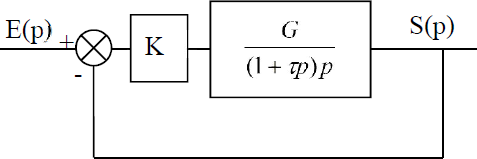
\includegraphics[width=\linewidth]{fig_02}
\end{marginfigure}


\begin{center}
\begin{tikzpicture}[xscale=16/10]
\tikzset{
semilog lines/.style={thin, bleuxp}, 
semilog lines 2/.style={semilog lines,bleuxpc},
semilog half lines/.style={semilog lines 2,dotted },
semilog label x/.style={semilog lines,below,font=\tiny,black},
semilog label y/.style={semilog lines,right,font=\tiny,black}
}
\begin{scope}[yscale=6/150]
\OrdBode{10}
\semilog{-3}{3}{-60}{20}

\BodeGraph[orangexp,samples=150,ultra thick]{-3:3}{-\SOAmp{1}{.1}{1}+\IntAmp{0.01}+\POAmp{1}{0.01}}

%\BodeAmp[orangexp,thin,samples=150]{-2:2}{\SOAmpAsymp{10}{0.2}{.9}}
%s\BodeAmp[orangexp,ultra thick,samples=150]{-2:2}{\SOAmp{10}{0.2}{.9}}
%\draw (-1.5,28) node {\footnotesize $20\log K$};
%\draw (1.1,10) node {\footnotesize $-$40 dB/d\'ecade};
%\draw [dashed,ultra thick,bleuxp] (-.08,-60) -- (-.08,25);
%\draw (-.08,-60)  node {\Huge $\cdot$} node [above right]{\footnotesize $\omega_0$};
\end{scope}
\begin{scope}[yshift=-4cm,yscale=1/90]
\UniteDegre
\OrdBode{45}
\semilog{-3}{3}{-90}{90}
\BodeArg[orangexp,samples=150,ultra thick]{-3:3}{-\SOArg{1}{.1}{1}+\IntArg{0.01}+\POArg{1}{0.01}}
%\BodeArg[orangexp,samples=100,thin]{-2:2}{\SOArg{10}{0.2}{.9}}
%\BodeArg[orangexp,ultra thick]{-2:2}{\SOArg{10}{0.2}{.9}}
\end{scope}
\end{tikzpicture}
\end{center}

\ifprof
\begin{center}
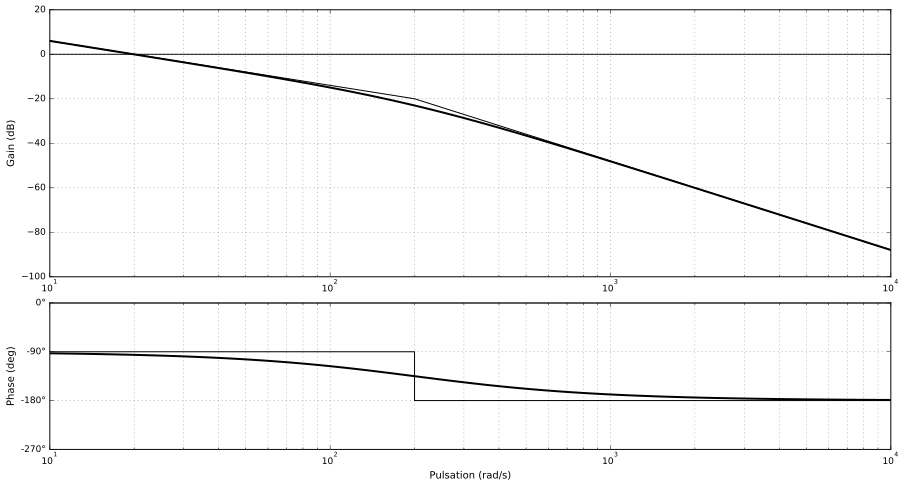
\includegraphics[width=\linewidth]{cor_01}

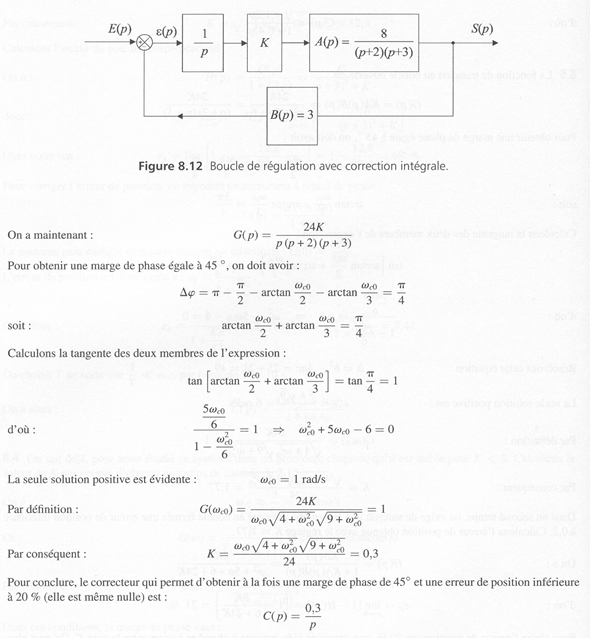
\includegraphics[width=\linewidth]{cor_02}

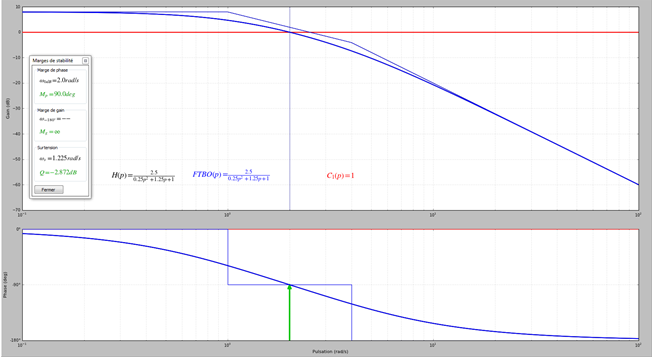
\includegraphics[width=\linewidth]{cor_03}

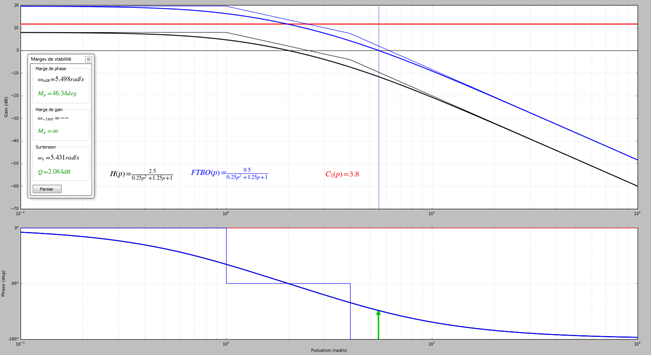
\includegraphics[width=\linewidth]{cor_04}
\end{center}
\else
\fi


\ifprof
\else
\begin{marginfigure}[-3cm]
\centering

\includegraphics[width=3cm]{Cy_02_Ch_01_Colle_02_qr}
\end{marginfigure}
\fi
